\documentclass[main.tex]{subfiles}
\begin{document}
    \chapter{Eddy Current Brakes}
    \label{ch:eddy-current-brakes}
    With only 1.3 kilometers of tube to work with, it is difficult to dissipate the kinetic energy at 100m/s quickly. Pure friction braking, as with the braking calipers (\refsec{sec:friction-braking-calipers}), cannot work alone, since either the enormous shear forces and heat generated will destroy the brakes, or the pod will not stop within the length of the tube. This is why Eddy Current (EC) brakes will be used for the braking. These permanent magnet eddy current brakes work by inducing an eddy current in the web of the aluminum rail. These eddy currents create an opposing magnetic field causing braking force on the pod. Most eddy current heat generation occurs in the rail, resulting in little heat addition to the pod system. This rate of heat generation will never come even within an order of magnitude of damaging the rail or the pod. The difficulty arises in the large forces that will be created by the brakes. The design of the brakes will have to be able to handle theses forces. 

    \section{Overall Design}
    For the brakes we will be using a pneumatic actuator and to do so we will be using the pneumatic circuit in \reffig{fig:pneumatic-circuit}. \\
    \begin{figure}[H]
        \centering
        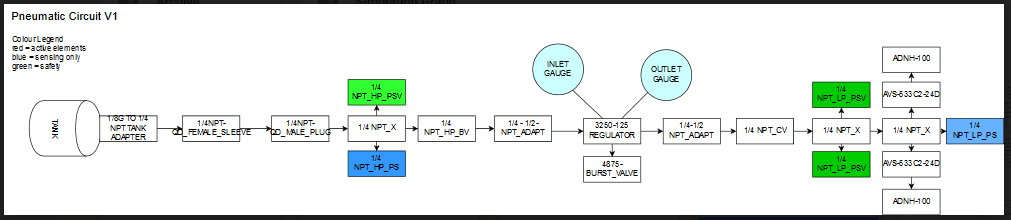
\includegraphics[width=\linewidth]{images/EC_Pnuematic_Circuit.png}
        \caption{EC Brakes Pneumatic Circuit Schematic that describes the overall system using proprietary part numbers.}
        \label{fig:pneumatic-circuit}
    \end{figure}
    
    The pneumatic circuit provides the actuation of the EC brakes, bringing them within effective range. Using two linear pneumatic actuators, the EC brakes are able to actuate along an axis towards the rail. The pneumatic actuator will be able to retract and extend, ensuring that the brakes remained dormant whilst in the acceleration phase and activated during the braking phase. The pneumatic circuit is electrically failsafe, utilizing solenoid valves to ensure that the brakes are extended and retracted during the correct velocity interval. The pneumatic actuators need to handle a large amount of lateral force created from the Eddy Current effect while braking at high speeds. Pneumatic actuators are do so very well because they can produce very large forces at low resource costs and do not require large mechanical assemblies, as it is a single component that achieves this. The pneumatic circuit is very similar in design to the one found in Friction Drive (\autoref{section:pneumatics}). The primary difference between these systems is that the actuators used in their assemblies are not the same.
    The tank will contain high pressure air at \SI{3000}{psi} and will contain the same safety and sensing elements as the pneumatic circuit seen on friction drive. As such, there will be a high-pressure tank and circuit that will be connected to a regulator which reduces the pressure into a low-pressure circuit. The MEOP of the high-pressure circuit will be \SI{3000}{psi} and the MEOP of the low-pressure circuit will be \SI{125}{psi}. Relief valves will be set at MEOP to ensure that the pressure does not exceed our expected values. This pneumatic circuit will also be proof tested in order to certify the MAWP of the system – which should be 1.5x the MEOP. \ref{fig:EC_Brake_Master_2018} shows the overall brake assembly. The piston is mounted to the frame through our piston mount which is attached to the magnet bar. Our brakes actuate back and forth in a straight line which is perpendicular to the rail. They keep their path due to linear rails that are also attached to the frame.
    \begin{figure}
    	\centering
        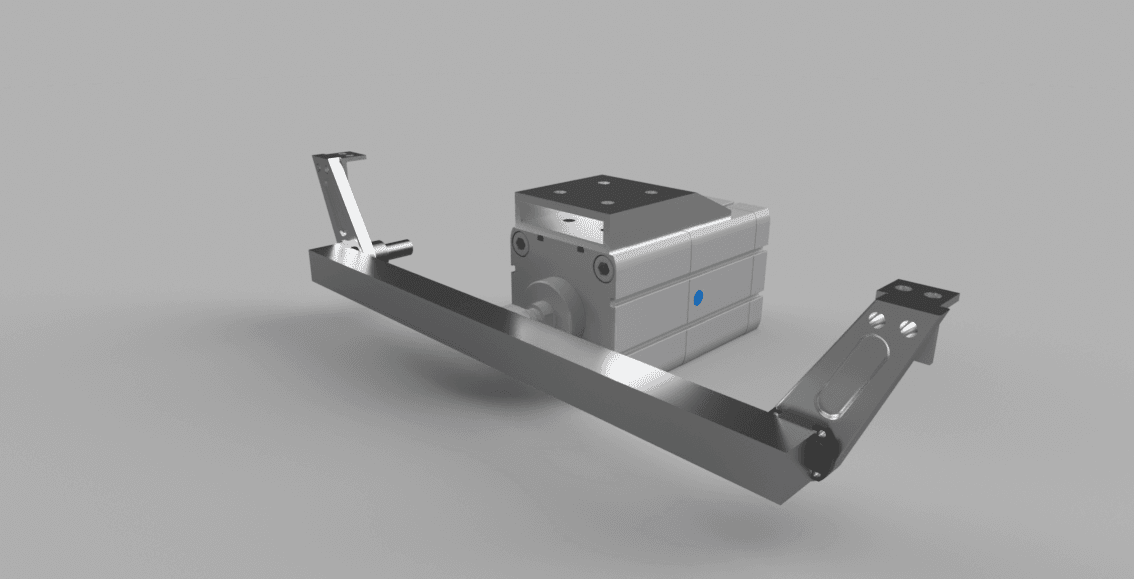
\includegraphics[width=\linewidth]{images/EC_Brake_Master_2018}
        \label{fig:EC_Assembly}
        \caption{The Master Assembly of the EC Brakes}
    \end{figure}

    A full Bill of Materials can be found in \reftab{tab:eddy-current-brakes-bom}.

    \section{Physical Modeling}
    \begin{table}
    	\centering
    	\begin{tabular}{@{}ll@{}} \toprule
            Parameters & Value\\ \midrule
            Dimensions(\si{m})     & 0.0254 $\times$ 0.0254 $\times$ 0.0254 \\
            Material     & NdFeB, Grade N52   \\
            Pull Force(\si{N})     & 165.34 \\
            Operating Temperature     & 353K  \\ \bottomrule
        \end{tabular}
        \caption{Magnet Specifications}
        \label{table:magnets}
    \end{table}
    Our eddy current brakes will be made with 2 arrays of 16 magnets (see \reftab{table:magnets} for magnet specifications) on either side of the rail. The array of magnets will be made using Halbach arrays, as seen in \reffig{fig:halbach-array}, which is a way of arranging magnets that increase the magnetic flux on one side of the array.\\

    \begin{figure}
        \centering
        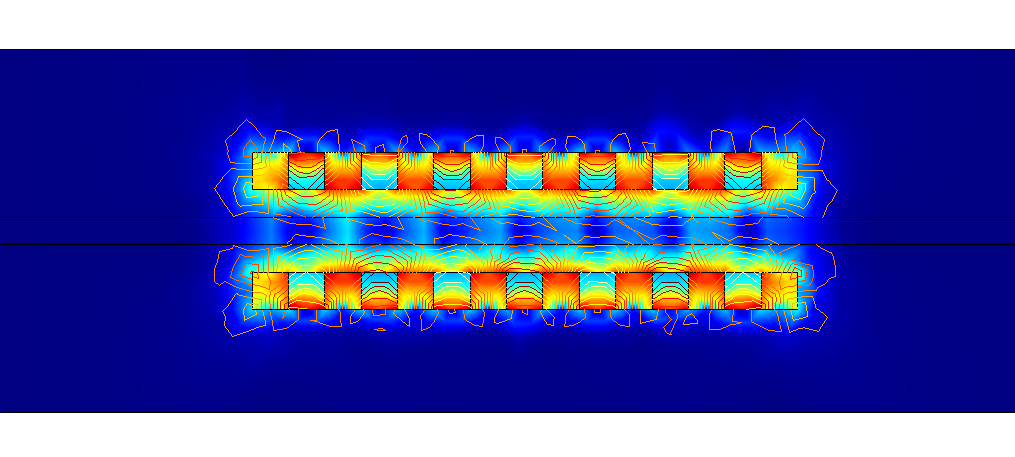
\includegraphics[width=\linewidth]{images/halbach_array.png}
        \caption{Halbach Array on the Rail}
        \label{fig:halbach-array}
    \end{figure}
     Since we are using magnets for the brakes there will be a force created both perpendicular and parallel to the actual rail. The equation for the lift force, which in this case is the force perpendicular to the rail.
     \begin{equation}\label{eq:lift-force}
     F_{\textrm{Lift}} = \frac{3\mu m^2}{32\pi z_0^4}\times\left(1 -\frac{\omega}{\sqrt[2]{v^2+\omega^2}}\right)
    \end{equation}
    Where $\mu$ is the vacuum permeability, m is the magnetic vertical dipole moment, $\omega$ is the velocity of magnetic propagation through the beam and $z_0$ is the separation of the magnets from the rail. While the magnitude of the drag force that will be created is given by
    \begin{equation}\label{eq:lift-force2}
    \left\lvert F_{drag}\right\rvert = \frac{\omega}{v} F_{lift}
    \end{equation}
     Using Equations \ref{eq:lift-force} and \ref{eq:lift-force2} we were able to graph the forces that we would expect from speeds between 0-\SI{100}{m/s} where $z_0 = \SI{19}{mm}$.\\

    \begin{figure}
        \centering
        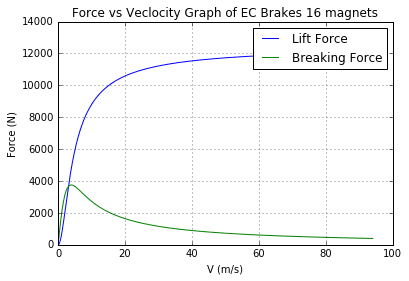
\includegraphics[width=\linewidth]{images/force_velocity_graph_16_magnets.png}
        \caption{Graph of the lift and drag forces experienced by the magnets, for one of the brakes}
        \label{fig:force-velocity-graph}
    \end{figure}
    Based on the graphs for force and velocity in \reffig{fig:force-velocity-graph}, we were able to determine the velocity profile, acceleration profile, and the distance profile.\\
    From the force graphs it becomes evident that the pod will have to endure large forces when braking. We can expect a maximum lift force of around \SI{14000}{N} and a maximum drag force of around \SI{4000}{N}. This means that the mounting to the frame and the position of the actuator need to be able to withstand these forces. The mounting points on the frame have been designed to be able to handle this force. The actuator is going to be oriented perpendicular to the rail. Initially we thought about angling the actuator, this way the actuator would only experience some of the total normal force and not its entirety. It was decided against this idea because this would require that we use an actuator with a larger stroke length. This would create a large bending moment which would not be ideal. As well the larger stroke length leads to the another problem of a large bending moment.
    From the acceleration time graph we can also see that at slower speeds, there is a spike in the total acceleration that the pod will feel. This acceleration comes to about 5Gs, which the pod is not designed to handle. Our pod has been designed to be able to safely handle 3Gs. To solve this problem we are going to be using our actuator to slowly retract the brakes at \SI{10}{m/s} at which point the low speed friction brakes would take over and slow the pod down to a complete stop.\\

   Taking that into account as well as the expected propulsion we now have a complete idea of what our displacement (\reffig{fig:distance-profile}), velocity (\reffig{fig:total-velocity-profile}) and acceleration profiles (\reffig{fig:total-acceleration-profile}) will look like.\\
   
    \begin{figure}
        \centering
        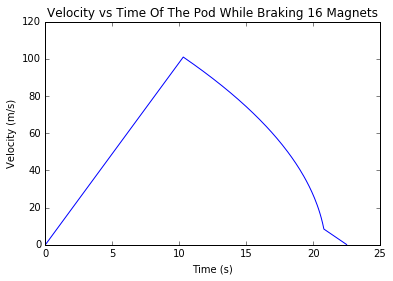
\includegraphics[width=\linewidth]{images/totalvelocityprofile}
        \caption{Velocity Profile for the entire journey of the pod.}
        \label{fig:total-velocity-profile}
    \end{figure}
    \begin{figure}
        \centering
        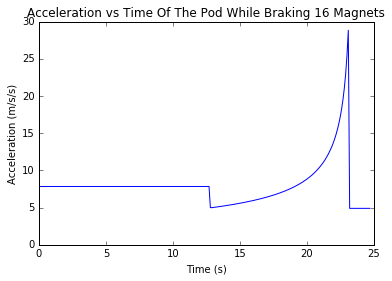
\includegraphics[width=\linewidth]{images/totalaccelerationprofile}
        \caption{The total acceleration profile for the pod. This includes the acceleration of the propulsion system all the way to the use of the friction brakes right at the end}
        \label{fig:total-acceleration-profile}
    \end{figure} 
    \begin{figure}
        \centering
        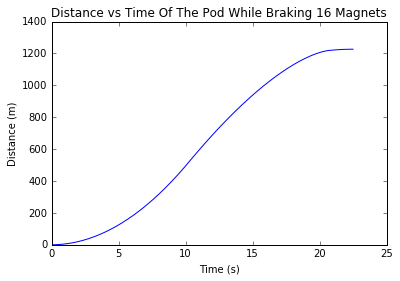
\includegraphics[width=\linewidth]{images/totaldistanceprofile}
        \caption{The total distance that the pod travels through all the phases of the trip.}
        \label{fig:distance-profile}
    \end{figure}
    
    Since we are using magnets, that means that there will always be a force related at some separation from the track. That means that when the brakes are in an off state they need to be far enough from the track such that the force that the pod experiences is minimal. In order to figure this out what we used the equation for drag force (\ref{eq:lift-force2}) and inputted separation values and determined the one that would give us the lowest maximum drag force that fit our design requirements. From that we found that the optimal distance was \SI{0.049}{mm} away from the track when deactivated.    
    
    \section{Thermal}
    One thing that we have to be careful of is the heating that the brakes would have. As stated in \reftab{table:magnets} the max operating temperature for the magnets is \SI{80}{\celsius} this means that we need to make sure that that the brakes do not get to that level.\\

    \begin{figure}
    	\centering
        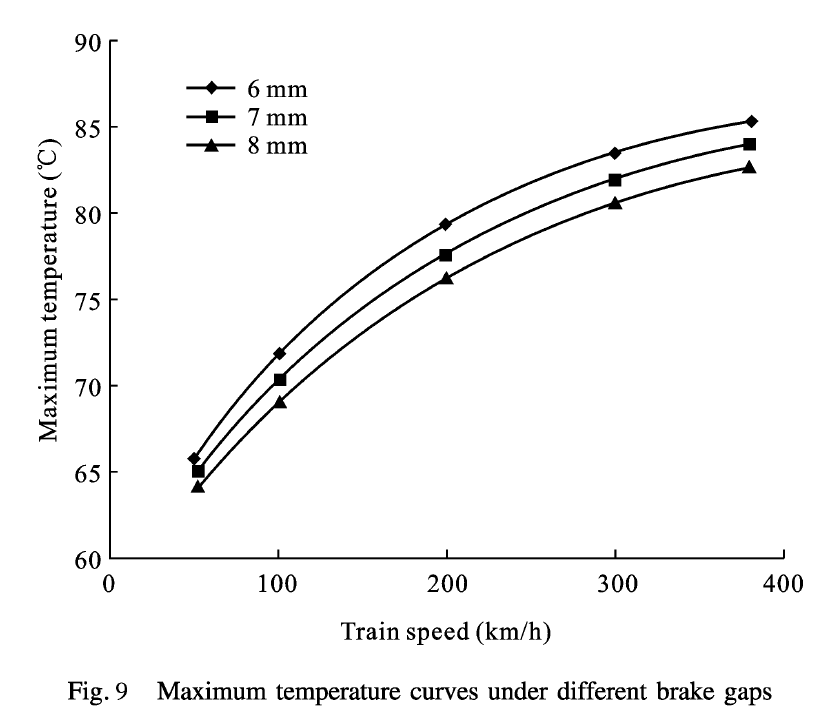
\includegraphics[width=\linewidth]{images/EC_heat}
        \caption{Maximum temperature curves under different brake gaps}
        \label{fig:ec-heat}
    \end{figure}
    \reffig{fig:ec-heat} shows how hot the rail would get at high speeds due to the Eddy Current brakes. For this plot we use a $z_0$ values of 6-\SI{8}{mm}. You can see that at \SI{100}{m/s}, which is the max speed our pod is designed for, the total heating on the rail ranges between 69-\SI{73}{\celsius} from this if we then extrapolate to the value of $z_0 = \SI{19}{mm}$ that we are using we see that the thermal heating due to the Eddy Current brakes will not damage the rail or the magnets in the brakes at all.

    \section{Structural}
    One thing that we have to understand is how these brakes will react in the case of failure, electrical or otherwise. The brakes require to power to activate, therefore in case of power failure in our main battery we have a backup battery specifically for the brakes that will activate and slow the pod down.  \\
    As seen in the force time graphs above \reffig{fig:force-velocity-graph} the brakes will experience large forces when the pod is at high speeds, and when braking at low speeds. We have already accounted for the low speed situation with the actuator. By relieving the brakes at \SI{10}{m/s} we avoid dealing with a jerk at the end of or run. So the main thing that needs to be looked at is the case when we are at high speed. To make sure that our pod is able to handle this we ran simulations on each part: the Piston mount (\reffig{fig:ECPiston}), the Shaft mount (\reffig{fig:ShafttMount}), and the Magnet bar (\reffig{fig:MagnetBar}).\\
    \begin{figure}
    	\centering
        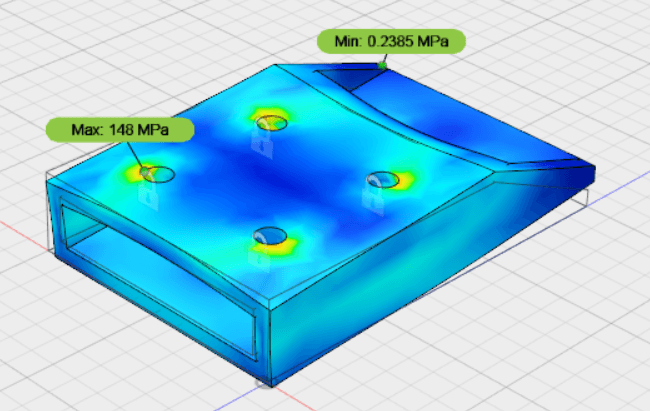
\includegraphics[width =\linewidth]{images/ECPistonMount}
        \caption{FEA of the Piston mount for the Eddy Current Brakes}
        \label{fig:ECPiston}
    \end{figure}
    \begin{figure}
    	\centering
        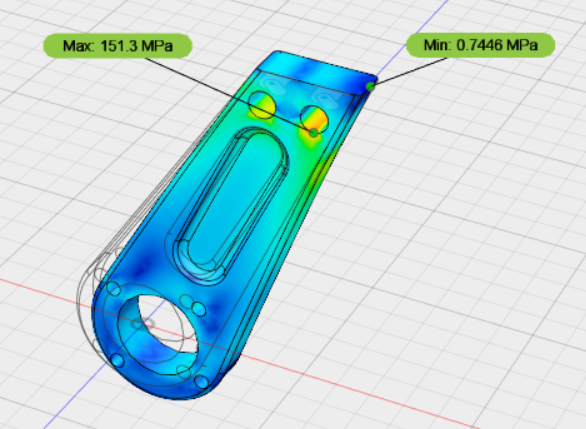
\includegraphics[width = \linewidth]{images/ShaftMount}
        \caption{FEA of the Shaft Mount for the Eddy Current Brakes}
        \label{fig:ShafttMount}
    \end{figure}
    \begin{figure}
    	\centering
        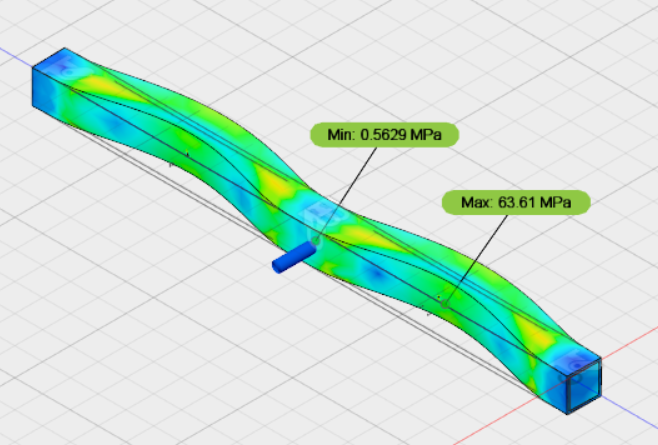
\includegraphics[width=\linewidth]{images/MagnetBarFEA}
        \caption{FEA of the Magnet Bar}
        \label{fig:MagnetBar}
    \end{figure}
    From our simulations we see that in our extreme case the brakes will be able to safely handle the forces.\\

    \section{Safety and handling}
    Neodymium magnets have the ability to damage both equipment and handlers. Therefore, only members of the team that have taken the magnet handling safety course are permitted access to the magnets. When transferring the magnets always hold two separate magnets in opposite hands away from any ferromagnetic metal. Eye protection must be worn when handling the magnets as magnet dust may get into eyes and gloves are recommended. In case of emergency evacuation, place magnets in a safe area away from ferromagnetic metals. 
    
\end{document}
